\section{Matrix Completion, Imputation}
Imputation or Matrix completion problems deal with missing observations. The most famous application is probably the Netflix prize, in which a very large, very sparse data matrix encodes the preferences of Netflix users. Missing entries correspond to the case where it is not known what a certain user might think of a movie.

\begin{figure}
\centering
    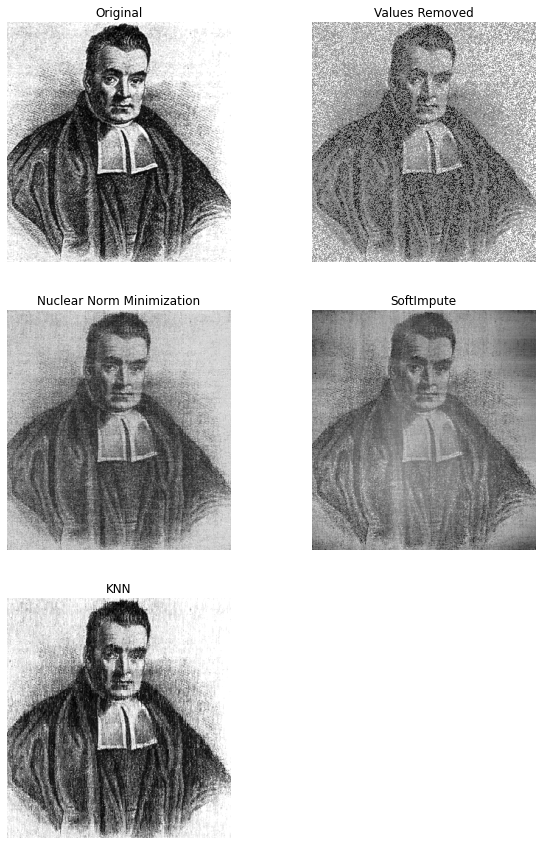
\includegraphics[width=0.7\textwidth]{impute_05.png}
    \caption{Results for different imputation methods reconstructing the image of the man rumored to be Bayes himself after 50\% of the pixels are removed.}
    \label{fig:impute_05}
\end{figure}


\subsection{Nuclear Norm Regularization}
Given a matrix $\mathbf{X}\in\mathbb{R}^{m\times n}$, in which observed entries are indexed by the set $\Omega = \{(i,j) : X_{i,j}\mathrm{\ is\ observed.} \}$\cite{hastie2015matrix}. Define the projection $P_{\Omega}(\mathbf{X}) \in \mathbb{R}^{m\times n}$ to be the matrix so that $P_{i,j} = X_{i,j}\ \forall\ (i,j) \in \Omega$ and $P_{i,j} = 0\ \mathrm{if\ }(i,j)\notin\Omega$, which is to say: take the matrix $\mathbf{X}$ and set all the unobserved entries to $0$. 

Nuclear norm regularization corresponds to expressing completing $\mathbf{X}$ in terms of the convex optimization problem:

\begin{equation}
\argmin_{\mathbf{M}} H(\mathbf{M}) = \frac{1}{2}||P_{\Omega}(\mathbf{X-M})||^2_F + \lambda ||\mathbf{M}||_{*}
\end{equation}

Where $||\cdot||_{*}$ is the nuclear norm of $\mathbf{M}$ (cf. section \ref{sec:nuclearnorm}). The loss function is a tradeoff between accurately reproducing $\mathbf{X}$ and doing so with as low a rank as possible. Except, using the rank of $\mathbf{M}$ would make the optimization non-convex, so instead the nuclear norm is used, which is the sum of the singular values. Solving this problem is computationally still quite expensive, but is a lot of work on solving this problem for large datasets, for example \texttt{softImpute}, texttt{softImpute+}, which use soft-singular value thresholding that amounts to leveraging lower-rank representations of the data \cite{mazumder2010spectral}.